% !TEX encoding = UTF-8 Unicode
\subsection{Fase PROB: Progettazione Requisiti Obbligatori}
	\textbf{Periodo}: dal \insdate{16}{03}{2015} al \insdate{08}{04}{2015} \\Questa fase comincia con la fine della \insphase{Fase PA} e termina con l'incontro con il proponente al fine di mostrare il prototipo con i requisiti obbligatori sviluppati.\\Le attività di questa fase saranno le seguenti:
	\begin{itemize}
		\item\textbf{Definizione di Prodotto}: viene steso il documento \insdoc{Definizione di Prodotto v1.00}. Esso definisce la struttura interna del sistema e le relazioni dei componenti del prodotto relativi ai requisiti obbligatori.
		\item \textbf{Codifica}: con quest'attività inizia lo sviluppo da parte dei programmatori dei requisiti obbligatori. Sarà dunque seguito quanto riportato nel documento \insdoc{Definizione di Prodotto v1.00};
		\item \textbf{Esecuzione test}: verranno eseguiti automaticamente tutti i test di unità previsti dal documento \insdoc{Piano di Qualifica v 4.00};
		\item\textbf{Manuale Utente e Manuale Amministratore}: comincia la stesura dei manuali che forniranno indicazioni agli utilizzatori del sistema.
		\item\textbf{Incremento e Verifica Documenti}: vengono eseguite modifiche ai documenti già scritti, se necessario.
		\item\textbf{Glossario}: vengono aggiunti al file \insfile{Glossario.xml} i vocaboli dei quali si ritiene necessaria una definizione formale. Alla fine di questa fase vieni quindi generato il documento \insdoc{Glossario v4.00}.
	\end{itemize}
	\subsubsection{Diagramma di Gantt delle attività}
	\begin{figure}[H]\centering
		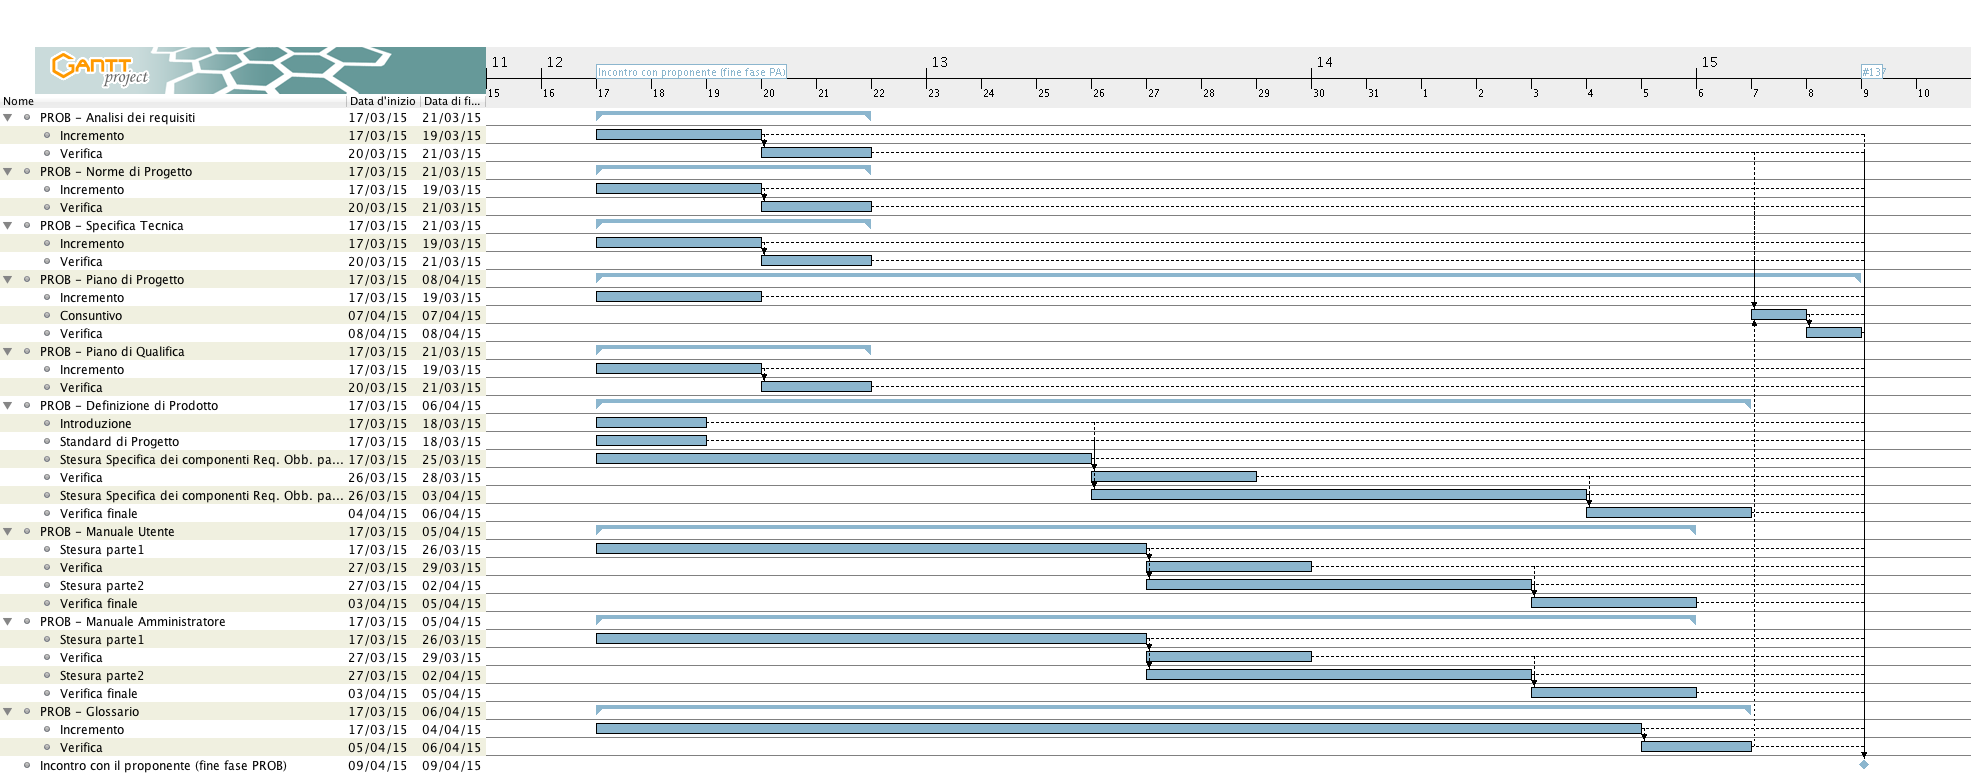
\includegraphics[width=\textwidth]{PianoDiProgetto/Pics/FasePROB.png}
	\caption{Gantt Fase PROB}
\end{figure}